\documentclass[a4paper,12pt]{article}

\usepackage[spanish, activeacute]{babel} 
\usepackage{amsmath}
\usepackage{amsfonts}
\usepackage{amssymb}
\usepackage{graphicx}

\begin{document}

\tableofcontents
\pagebreak

\section{Autorizaci'on}

\pagebreak

\section{Resumen}

\pagebreak

\section{Palabras clave}

\pagebreak

\section{Introducci'on}

\pagebreak

\section{Especificaci'on de requisitos}

	\subsection{Descripci'on general}

	\subsection{Requisitos de interfaces externas}

	\subsection{Requisitos no funcionales}

	\subsection{Requisitos funcionales}

	\subsection{Coste econ'omico}

\pagebreak

\section{Casos de uso}

	\subsection{Inicio de sesi'on}
		\emph{\underline{Objetivo:}}\bigskip \\Se inicia la sesi\'on con el PDA abri\'endose as\'i la aplicaci\'on. Al iniciar la sesi\'on ser\'a necesario que el usuario introduzca su clave y nombre de usuario, que de ser correctos le dar\'an acceso a los men\'us.\bigskip \\ \emph{\underline{Entradas:}}
\begin{itemize}
\item Clave de usuario.
\item Nombre de usuario.
\end{itemize}
\emph{\underline{Precondiciones:}}\bigskip \\No hay precondiciones.\bigskip \\ \emph{\underline{Salidas:}}\bigskip \\En caso de \'exito (clave y nombre de usuario son correctos): 
\begin{itemize}
	\item Se muestra el men\'u de la aplicaci\'on en la pantalla del PDA.
\end{itemize}
En caso de fallo (clave y nombre de usuario no son correctos): 
\begin{itemize}
	\item Se informa al usuario de que los datos introducidos no son correctos.
	\item Se vuelve a la pantalla de inicio para que el usuario tenga la posibilidad de volver  a intentar iniciar la sesi'on.
\end{itemize}
\emph{\underline{Postcondici\'on si \'exito (clave y nombre de usuario son correctos):}}\bigskip \\Se muestra el men\'u de la aplicaci\'on por la pantalla del PDA.\bigskip \\ \emph{\underline{Postcondici\'on si fallo (clave y nombre de usuario no son correctos):}}\bigskip \\ Se informa al usuario de que los datos introducidos no son correctos y se le ofrece la posibilidad de intentar acceder a la aplicaci\'on de nuevo.\bigskip \\ \emph{\underline{Actores: }}
\begin{itemize}
	\item Usuario con PDA.
	\item Servidor del hospital.
	\item PDA.
\end{itemize}

\emph{\underline{Secuencia normal:}}
\begin{enumerate}
	\item Al encender el PDA, se solicita al usuario que introduzca su clave y su nombre de usuario y \'estos son enviados a la base de datos del servidor del hospital para que sean verificados.
	\item El servidor busca en su base de datos la clave y el nombre de usuario que se acaban de introducir para confirmar que est\'a iniciando sesi\'on una persona autorizada, personal del hospital. En caso de que la b\'usqueda tenga \'exito pasar a 3, en caso contrario pasar a E1.
	\item Una vez confirmada la clave y el nombre de usuario, en el PDA tenemos disponible el men\'u con todas las posibles operaciones que se pueden realizar con la aplicaci\'on.
\end{enumerate}

\emph{\underline{Secuencias alternativas:}}\bigskip \\ E1.- Se informa al usuario de que los datos que ha introducido no son correctos y se le da la oportunidad de volver a introducirlos (paso 1). \bigskip \\ Para ilustrar mejor est'a secuencia de acciones, incluimos el diagrama de secuencia de este caso de uso (Figura \ref{fig:inicio_sesion})

\begin{figure}[thb]
	\begin{center}
		\framebox{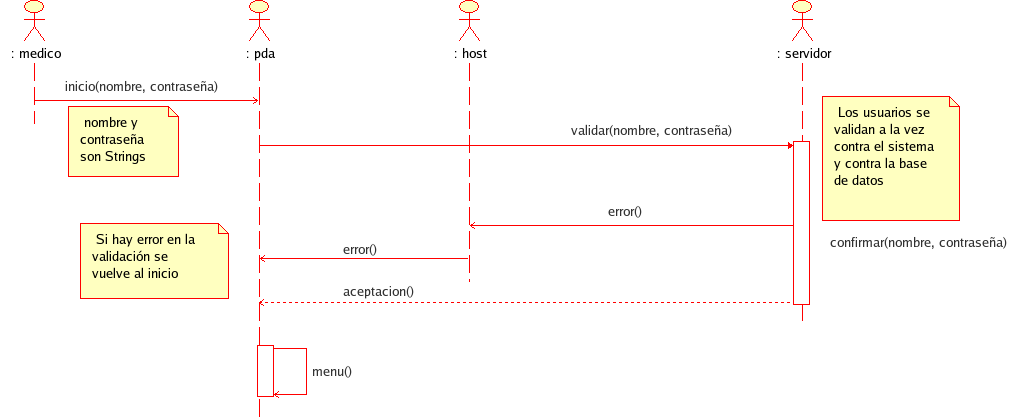
\includegraphics[scale=0.4]{dsecuenciainicio.png}}
     	\end{center}
    	\caption{Diagrama de secuencia del inicio de sesi'on}\label{fig:inicio_sesion}
\end{figure}

	\subsection{Impresi'on de documentos}
		\emph{\underline{Objetivo:}}\bigskip \\ El personal sanitario, dotado de un PDA, solicita la impresi\'on de un documento de un paciente que se encuentre disponible en la base de datos del hospital. Dicha impresi\'on se realizar'a por la impresora m\'as cercana al lugar en el que se ha solicitado \'esta.\bigskip \\ \emph{\underline{Entradas:}} 
\begin{itemize}
\item Documento a imprimir.
\item Nombre del paciente del que solicitamos el documento a imprimir.
\end{itemize}

\emph{\underline{Precondiciones:}}\bigskip \\ Los documentos que se solicitan imprimir deben encontrarse en la base de datos del hospital as'i como el paciente, que tambi'en debe estar registrado en la base de datos.\bigskip \\ \emph{\underline{Salidas:}}\bigskip \\ En caso de \'exito: 
\begin{itemize}
	\item Confirmaci\'on de la solicitud aceptada.
	\item Impresora por la que se va a realizar el trabajo.
	\item Documento imprimido en la impresora indicada.
\end{itemize}
En caso de fallo: 
\begin{itemize}
	\item Se informa al usuario de la imposibilidad de realizar la petici\'on.
\end{itemize}

\emph{\underline{Postcondici\'on si \'exito:}}\bigskip \\ Se realiza la impresi\'on por la impresora m\'as cercana.\bigskip \\ \emph{\underline{Postcondici\'on si fallo:}}\bigskip \\ Se informa de que no se ha podido realizar la impresi\'on y se vuelve al men'u principal.\bigskip \\ \emph{\underline{Actores: }}
\begin{itemize}
\item Usuario con PDA.
\item Servidor del hospital.
\item Cola de impresi\'on de las impresoras del centro.
\item PDA.
\end{itemize}

\emph{\underline{Secuencia normal:}} 
\begin{enumerate}
\item El usuario solicita al servidor la impresi\'on de un documento concreto de un paciente del hospital desde su PDA. Si error al conectar con el servidor pasa a E1, sino pasa a 2.
\item El servidor busca en su base de datos el documento que queremos imprimir. Si lo encuentra pasa a 3, sino pasa a E1.
\item El servidor calcula la posici\'on del PDA y en funci\'on de ella devuelve la impresora m'as cercana,  la elegida para imprimir el documento.
\item El servidor manda el documento a la cola de la impresora m\'as cercana.
\item El servidor envia al PDA la confirmaci\'on de impresi\'on aceptada, informando de cual es la impresora que en la que se realiza la tarea.
\item Volvemos al men'u principal.
\end{enumerate}

\emph{\underline{Secuencias alternativas:}}\bigskip \\E1.- Se informa al usuario de que no se puede realizar la impresi'on en ese momento y se le invita a intentarlo m\'as tarde. Volvemos al men'u principal.\bigskip \\ Para ilustrar mejor est'a secuencia de acciones, incluimos el diagrama de secuencia de este caso de uso (Figura \ref{fig:cu_imprimir})

\begin{figure*}[h!]
	\begin{center}
        		\framebox{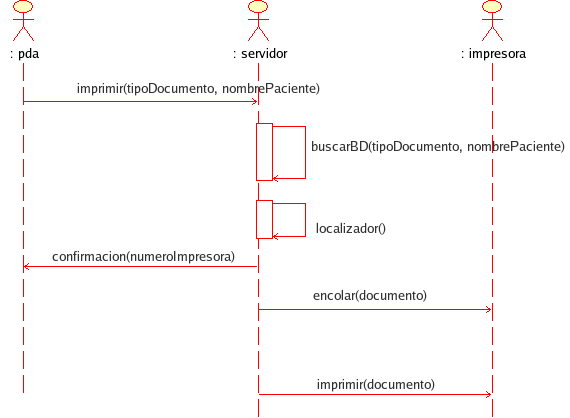
\includegraphics[scale=0.4]{dsecuenciaimprimir.png}}
     	\end{center}
    	\caption{Diagrama de secuencia de impresi'on de documentos}\label{fig:cu_imprimir}
\end{figure*}

	\subsection{Consulta de expedientes}
		\emph{\underline{Objetivo:}}\bigskip \\ Visualizaci'on por la pantalla del PDA del expediente de un paciente del hospital.\bigskip \\ \emph{\underline{Entradas:}}
\begin{itemize}
\item Nombre del paciente del que queremos consultar el expediente.
\end{itemize}

\emph{\underline{Precondiciones:}}\bigskip \\ El propietario del expediente que queremos visualizar debe ser un paciente registrado en la base de datos del hospital.\bigskip \\ \emph{\underline{Salidas:}}\bigskip \\ En caso de \'exito (el nombre paciente se encuentra en la base de datos del hospital): 
\begin{itemize}
	\item Se muestra en la pantalla del PDA el expediente del paciente solicitado.
\end{itemize}

En caso de fallo (el nombre paciente no se encuentra en la base de datos del hospital): 
\begin{itemize}
	\item Se informa al usuario de la imposibilidad de visualizar la informaci'on solicitada.
	\item Se vuelve al men'u principal.
\end{itemize}

\emph{\underline{Postcondici\'on si \'exito (el nombre paciente se encuentra en la base de datos del hospital):}}\bigskip \\ Se muestra el expediente del paciente solicitado en la pantalla del PDA.\bigskip \\ \emph{\underline{Postcondici\'on si fallo (el nombre paciente no se encuentra en la base de datos del hospital):}}\bigskip \\ Se informa al usuario de la imposibilidad de visualizar los datos solicitados y se vuelve al men'u principal.\bigskip \\ \emph{\underline{Actores: }}
\begin{itemize}
	\item Usuario con PDA.
	\item Servidor del hospital.
	\item PDA.
\end{itemize}

\emph{\underline{Secuencia normal:}}
\begin{enumerate}
	\item El usuario solicita al servidor la consulta del expediente de un paciente del hospital desde su PDA.
	\item El servidor busca en su base de datos el expediente del paciente solicitado. En caso de que la b\'usqueda tenga \'exito pasar a 3, en caso contrario pasar a E1.
	\item Se hace una lectura del expediente solicitado y se env'ia al PDA, mostr'andose por pantalla.
	\item Volvemos al men'u principal.
\end{enumerate}

\emph{\underline{Secuencias alternativas:}}\bigskip \\ E1.- Se informa al usuario del error en la consulta y se vuelve al men'u principal.\bigskip \\ Para ilustrar mejor est'a secuencia de acciones, incluimos el diagrama de secuencia de este caso de uso (Figura \ref{fig:consulta_expediente})

\begin{figure*}[h!]
	\begin{center}
        		\framebox{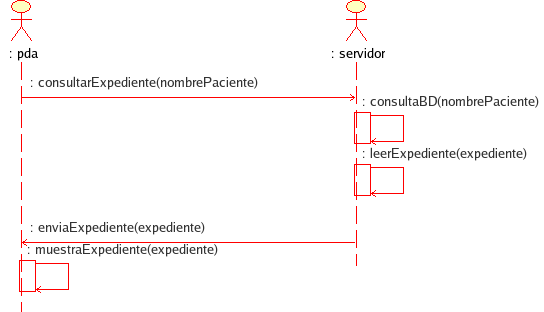
\includegraphics[scale=0.4]{consultar_expediente.png}}
     	\end{center}
    	\caption{Diagrama de secuencia de consultar expediente}\label{fig:consulta_expediente}
\end{figure*}		

\pagebreak

\section{Implementaci'on}

	\subsection{Tecnolog'ias}

	\subsection{Dise'no}

\pagebreak

\section{An'alisis del sistema}

	\subsection{Triangulaci'on}

	\subsection{Algoritmo de Floyd}

	\subsection{Conexi'on PDA-Servidor}

\pagebreak

\section{Manual de usuario}

\pagebreak

\section{Valoraci'on}

\pagebreak

\section{Ap'endices}

	\subsection{J2ME}

	\subsection{XML-RPC}

	\subsection{Algoritmo de Floyd}

\pagebreak

\begin{thebibliography}{XXX}

	\bibitem{Froute}J2ME Java 2 Micro Edition. Manual de usuario y tutorial.Agust'in Froute Quintas, Patricia Jorge C'ardenes. Ed. Ra-Ma.
	\bibitem{sun}http://java.sun.com
	\bibitem{kxmlrpc}http://kxmlrpc.objectweb.org
	\bibitem{eclipseme}  http://eclipseme.sourceforce.net

\end{thebibliography}

\end{document}